\section{Challenges}

\subsection{Non-Interpretable Latent Representations}

The randomness and inscrutability of the learning processes in neural networks has sparked interest in research pertaining to learning interpretable latent representations \citep{chen2016infogan}. Neural networks have proven to be highly capable function approximators in the general machine intelligence literature over the past couple of decades. However, without any explicit additional regularization over the latent variables, they are learned in an arbitrary manner to optimize over a user-defined convex loss function.

Due to this non-explainability of the weights of neural networks, they have been used as a black-box in practice. However, the non-explainability hampers their adoption in use-cases requiring explicit audits for accountability, and for humans to reason about why a system chose a particular outcome over the other options available. We believe that the disentanglement of the learned weights of a neural network is an important step in the direction toward addressing this shortcoming. This is achieved by using available labels to force representation learning to adhere to a predefined separation scheme in the latent space. To avoid the burden of requiring manually labelled data, we can use weakly supervised data. For example, product or service review ratings can be used as indicators of sentiment in text.

\subsection{Quantitative Evaluation of Language Quality}

The evaluation of novel generated text to measure its perceived quality, naturalness, fluency and compliance with predefined attributes, like sentiment, tense etc. is particularly important in tasks like ours where having parallel corpus as a gold set is not possible.

For the presence of certain attributes like sentiment, tense, formality, etc., it is fairly simple to devise a classification model that is trained on a large corpora of samples labelled as such. However, it is much more difficult to unambiguously state what makes a body of text more fluent or natural than another with mathematical rigour using quantitative metrics. Unsurprisingly, contemporary works in this area use human annotators \citep{hu2017toward,shen2017style,fu2017style} to gauge model success. However, this is not scalable to large sets of generated sentences, and researchers need to account for subjectivity and inter-annotator agreement to further normalize scores obtained from human assessments \citep{bermingham2009study,nowak2010reliable}.

To offset this problem, while still avoiding the need for human annotators to evaluate the target text, we have used metrics like sentence embedding similarity as proposed by \cite{fu2017style}. In this method, we compute sentence embeddings, augmented by the removal of words that are highly correlated with any specific label, and use it to assess content preservation. We also use a Kneser-Ney smoothed \citep{kneser1995improved} language model to evaluate fluency. All the quantitative metrics we use are described in greater detail in Section \ref{sec:evaluation-metrics}.


\section{Model Overview}

We provide a novel approach to solve this open problem of non-interpretable latent representations in neural networks. We juxtapose this approach and its experimental results against the current state-of-the-art models. We empirically demonstrate the separation of content and style spaces by visualizing the inferred spaces of labelled sentences in sentiment-transfer tasks, where the positive sentences in the test set are converted to equivalent sentences with a negative sentiment, and vice-versa. This model is also generalizable to problems involving multiple classes, like style transfer by authors, artists, topic, etc. using its standard implementation.

Our model is built upon an autoencoder with a sequence-to-sequence (Seq2Seq) neural network \citep{sutskever2014sequence}, as described in Section \ref{sec:seq2seq-objective}. This is our base model, the objective function of which is to simply reconstruct the input text. We implement our model using both a deterministic autoencoder \citep{baldi2012autoencoders} as well as a variational autoencoder \citep{kingma2013auto}.

Then we introduce two auxiliary losses, multi-task label classification loss and a style discriminative adversarial loss in Sections \ref{sec:multitask-classification-objective} and \ref{sec:adversarial-style-objective}, respectively. In addition to these auxiliary losses, we propose a novel bag-of-words adversarial loss in Section \ref{sec:adversarial-bow-objective}. This makes our model a dual-adversary model. We also propose a novel style dropout regularization to improve the content space encoding. Section \ref{sec:generating-novel-text} presents the approach to transfer style while generating novel text.

Figures \ref{fig:model-overview-training} and \ref{fig:model-overview-inference} depict the training and generation processes of our approach.

\begin{figure}[ht]
	\centering
	\includegraphics[width=\linewidth]{images/model-overview-training}
	\caption{Model Training Overview}
	\label{fig:model-overview-training}
\end{figure}

\begin{figure}[ht]
	\centering
	\includegraphics[width=\linewidth]{images/model-overview-inference}
	\caption{Model Inference Overview}
	\label{fig:model-overview-inference}
\end{figure}


\section{Autoencoder} \label{sec:seq2seq-objective}

An autoencoder encodes an input to a latent vector space, from which it decodes the input itself. By doing so, the autoencoder learns meaningful representations of data. This serves as our primary learning objective. Besides, we also use the autoencoder weights for text generation in the attribute style-transfer application.

Let $x=(x_1, x_2, \cdots x_n)$ be an input sentence. The encoder encodes $x$ using a recurrent neural network (RNN) with gated recurrent units (GRU) \citep{cho2014learning}. It obtains a hidden state $\bm h$, which in our formulation, is two separate spaces, $\bm s$ for style and, $\bm c$ for content. This variation on how the latent space is parameterized still requires an equal number of parameters when compared to a vanilla RNN encoder. Then a decoder RNN generates a sentence, which ideally should be $x$ itself. Suppose at a time-step $t$, the decoder RNN predicts the word $x_t$ with probability $p(x_t | \bm h, x_1 \cdots x_{t-1})$, then the autoencoder is trained by minimizing a cross-entropy loss between the input sequence and the generated sequence. The training process is described in more a detailed manner as follows:

The encoder produces the style and content, given that $\theta_{E_s}$ represents the subset of encoder parameters responsible for the production of the style vector and $\theta_{E_c}$, similarly, represents the encoder responsible for the production of the content vector.
\begin{align*}
	\bm s =
	 & \theta_{E_s}(x) \nonumber \\
	\bm c =
	 & \theta_{E_c}(x) \nonumber
\end{align*}

Following which, the decoder attempts to predict the original distribution of $x$ by computing the softmax over the vocabulary size, for as many time-steps as the sequence length, as shown in Equation \ref{eqn:dae-rec}
\begin{equation} \label{eqn:dae-rec}
	\mathcal{L}_\text{rec}(\bm\theta_E,\bm\theta_D)= -\mathbb{E}[log p_D(x|\bm s, \bm c)]
\end{equation}
where $\bm\theta_E$ and $\bm\theta_D$ are the parameters of the encoder and decoder, respectively. Since this loss trains the autoencoder to reconstruct $x$, it is also called the reconstruction loss.


\subsection{Variational Autoencoder}

In addition to the deterministic auto-encoding objective presented above, we also implement a variational autoencoder. The variational sampling and KL divergence losses are applied for both the style space $\bm s$ and the content space $\bm c$, separately. The weights applied to each KL divergence loss are tuned independently as a hyperparameter.

Equation \ref{eqn:vae-rec} shows the reconstruction objective that is minimized by the model in the VAE variant of our model.

\begin{align} \label{eqn:vae-rec}
	\mathcal{L}_\text{rec}(\theta_D, \theta_E; x) = \nonumber
	 & - \mathbb{E}_{q_{E_s}(\bm s|x) q_{E_c}(\bm c|x)} [log p_D(x|\bm s, \bm c)] \nonumber \\
	 & + \lambda_{\text{skl}} KL(q_{E_s}(\bm s|x)||p(z)) \nonumber                          \\
	 & + \lambda_{\text{ckl}} KL(q_{E_c}(\bm c|x)||p(z))
\end{align}
where $\lambda_{\text{skl}}$ and $\lambda_{\text{ckl}}$ are the weights for each of the KL divergence terms.

The motivation for using a variational autoencoder variant to compare the base deterministic autoencoder model to, is the property of VAEs that enable them to learn smooth and continuous latent spaces, without many dead zones in the latent space that cannot be decoded from. \cite{bowman2016generating} show this empirically by using the latent space of a text variational autoencoder to interpolate between and generate novel sentences from the latent spaces between two valid sentences from a corpus.

Since our objective is to use empirically inferred latent vectors to eventually achieve the attribute style transfer objective, it would be beneficial to compare the experimental performance of a variational autoencoder against a deterministic autoencoder.


Besides the above reconstruction losses, we design auxiliary losses to disentangle the latent space such that $\bm h$ can be separated into two spaces $\bm s$ and $\bm c$, representing style and content respectively, i.e., $\bm h = [\bm s ; \bm c]$, where $[\cdot;\cdot]$ denotes concatenation. We also design additional regularizations on the latent space to encourage learning this disentangled representation.


\section{Multi-Task Classification} \label{sec:multitask-classification-objective}

Our first auxiliary loss ensures the style space does contain style information. We build a classifier trained using the style space $\bm s$ as its features, predicting the true style (label) $y$, which is a part of the training data.

This loss can be viewed as a multi-task objective, in addition to the original reconstruction objective, which ensures that the neural network not only decodes the sentence, but also predicts its style (e.g. sentiment) from a sub-space of the latent representation. Similar multi-task losses have been used in previous work for sequence-to-sequence learning \citep{luong2015multi}, sentence representation learning \citep{jernite2017discourse} and sentiment analysis \citep{balikas2017multitask}, among others.

In our application, we follow previous work \citep{hu2017toward,shen2017style,fu2017style} and treat the sentiment as the style of interest for our primary evaluation. However, since our model generalizes to more than one class, we uses a simple multi-layer perceptron (MLP) followed by a softmax distribution over the possible labels. The softmax function can be expressed as the following expression
\begin{equation*}
	\sigma(\mathbf{z})_j = \frac{e^{z_j}}{\sum_{k=1}^K e^{z_k}} \text{for} j \in {1, \cdots K}
\end{equation*}
where $z_j$ denotes an arbitrary label's unweighted probability and $K$ is the total number of labels in the training data. The softmax distribution is re-weighted such that it's constituent values sum up to 1, which is very useful to model probability predictions over an arbitrary number of classes.

The class distribution predicted by the discriminative classifier is given by
\begin{equation} \label{eqn:class-pred}
	p(y | \bm s; \bm\theta_\text{mult}) = \sigma(\bm w_\text{mult}^\top \bm s + b_\text{mult})
\end{equation}
where $\bm\theta_\text{mult}=[\bm w_\text{mult}; b_\text{mult}]$ are the classifier's parameters for multi-task learning.

This is trained using a simple cross-entropy loss.
\begin{equation} \label{eqn:multi-task-loss}
	\mathcal{L}_\text{mult}(\bm\theta_{E};\bm\theta_\text{mult}) =
	- \mathbb{E} [\log p(y | \bm s; \bm\theta_\text{mult})]
\end{equation}
where $\bm\theta_E$ are the encoder's parameters.


\section{Adversarial Style Discriminator} \label{sec:adversarial-style-objective}

The above multi-task loss only operates on the style space, but does not have an effect on the content space $\bm c$. With only the multi-task loss, we cannot guarantee that the encoder would not also encode stylistic features within the content space. We therefore apply an adversarial loss to disentangle the content space from style information, inspired by adversarial generation \citep{goodfellow2014generative}, adversarial domain adaptation \citep{liu2017adversarial}, and adversarial style transfer \citep{fu2017style}.

The main idea is to introduce an adversary that deliberately attempts to discriminate the label $y$ of training samples using only the content vector $\bm c$. Then the autoencoder is trained to learn a content vector space from which its adversary cannot predict style information. Concretely, the adversarial discriminator predicts style $y$ by computing a softmax distribution over a multi-layer perceptron's output layer.
\begin{equation}
	p(y | \bm c; \bm\theta_\text{dis}) = \sigma(\bm w_\text{dis}^\top \bm c + b_\text{dis})
\end{equation}
where $\bm\theta_\text{dis}=[\bm w_\text{dis}; b_\text{dis}]$ are the parameters of the adversary.

It is trained by minimizing the following objective
\begin{equation} \label{eqn:adv-disc-loss}
	\mathcal{L}_\text{dis}(\bm\theta_\text{dis}) =
	- \mathbb{E} [\log p(y | \bm c; \bm\theta_\text{dis})]
\end{equation}

The adversarial loss appears similar to the multi-task loss as in Equation \ref{eqn:multi-task-loss}. However, it should be emphasized that, for the adversary, the gradient is not propagated back to the autoencoder, i.e., $\bm c$ is treated as shallow features, as is evident from the omission of $\theta_{E}$ from the training parameters. The only adversarial component is the loss itself. The network parameters are mutually exclusive for the autoencoder and the adversarial discriminator.

Having trained an adversary, we would like the autoencoder to learn latent representations, such that $\bm c$ is not discriminative in terms of the style or attribute we want to transfer. In other words, we penalize the entropy of the adversary's prediction, given by
\begin{equation}
	\mathcal{L}_\text{adv}(\bm\theta_E) = \mathcal{H}(p_\text{dis}(y | \bm c))
\end{equation}
where $\mathcal{H}=-\sum_{i\in\text{labels}} p_i\log p_i$ is the empirical Shannon entropy of the distribution. The adversarial objective is maximized, in this phase, with respect to the encoder. The motivation behind this objective is to increase the uncertainty of the discriminative classifier with respect to predicting style from the content vector. The maximum entropy value attainable over the distribution of attributes is the point at which each label is predicted with equal-probability i.e. the highest uncertainty.


\section{Adversarial Bag-of-Words Discriminator} \label{sec:adversarial-bow-objective}

In addition to the auxiliary losses used above, we also propose a novel bag-of-words discriminator on the style space. The motivation for having this objective is to try and emulate the adversarial signal provided by the style discriminator, and do the same for the content. Here, we define the content of the sentence as the words from the original sentence without any words that are discriminative of style. The input sentences $x$ are represented as a vector of the same size as the corpus vocabulary, with each index of the vector a discrete probability of a word's presence in the sentence. Therefore, this bag-of-words representation is comprised of only 1s and 0s.

The bag-of-words discriminator uses the style vector $\bm s$ produced by the autoencoder model and tries to predict the true bag-of-words distribution using a set of parameters that are distinct from those of the autoencoder. The discriminator uses a logistic regression to predict a probability of each word's occurrence in the original sentence, between 0 and 1.
\begin{equation}
	p(b | \bm s; \bm\theta_\text{bow}) = \sigma(\bm w_\text{bow}^\top \bm s + b_\text{bow})
\end{equation}

This objective is trained in a similar method to the style adversary, by using a cross-entropy loss
\begin{equation} \label{eqn:adv-bow-disc-loss}
	\mathcal{L}_\text{bow}(\bm\theta_\text{bow}) =
	- \mathbb{E} [\log p(b | \bm c; \bm\theta_\text{bow})]
\end{equation}
We also refrain from propagating the effects of this discriminator loss $\mathcal{L}_\text{bow}$ to the encoder parameters, ensuring that the parameters that each adversary and the encoder can update are mutually exclusive.

Similar to the style adversary, the empirical Shannon entropy of the predicted distribution is provided as a training signal for the autoencoder model to maximize.
\begin{equation}
	\mathcal{L}_\text{badv}(\bm\theta_E) = \mathcal{H}(p_\text{bow}(b | \bm s))
\end{equation}

The motivation for this adversarial loss is similar to the one used in the context of the style discriminator. We want to encourage the encoder to learn a representation of style that the bag-of-words discriminator cannot predict most of the original words from.

\subsection{Lexicon Augmented Discriminator}

An improvement to the bag-of-words discriminator could be made assuming the availability of a lexicon of words that are associated with a high probability with each of the styles that we are trying to disentangle.  A bag-of-words representation that excludes these words can now be created, such that the size of each representation is the set difference given by $(\text{\# vocab words}) \setminus (\text{\# lexicon words})$.

Our motivation for this enhancement is to avoid penalizing the autoencoder model for encoding words that are pertinent and discriminative for style that may be encoded in the style space. For the sentiment task in our experiments, we use a lexicon of positive and negative sentiment words curated by \cite{hu2004mining}.


\section{Style Dropout Regularization} \label{sec:style-dropout}

In addition to the regular training objectives, we also describe a novel regularization technique for disentanglement tasks. This method can also be viewed as analogous to a training objective like the bag-of-words loss.

In our model, we describe the main adversarial loss for style disentanglement by training a discriminator on the content space. However, there is a possibility of the autoencoder learning to ignore the content vector during generation entirely and using only the style space for encoding and later decoding the salient features of the corpus. This scenario is depicted in Figure \ref{fig:model-content-bypass} and can be thought of as the model bypassing the content space due to the presence of an adversary that penalizes any style signal in the content space $\bm c$.

\begin{figure}[ht]
	\centering
	\includegraphics[width=\linewidth]{images/model-content-bypass}
	\caption{Content Space Bypassing}
	\label{fig:model-content-bypass}
\end{figure}

To address this issue, we propose a customized version of Dropout \citep{srivastava2014dropout}. Similar to how each neuron in a network is dropped out with a predefined probability in the general version of dropout, in this version, we drop out entire style vectors in the mini-batch randomly with a predefined probability. The motivation for doing this is to reinforce the fact that the content latent vector is not to be ignored for the auto-encoding task despite the negative training signal from the adversary.


\section{Training Process} \label{sec:training-process}

The overall loss $\mathcal{L}_\text{ovr}$ used for the autoencoder is thus comprised of four different objectives: the reconstruction objective, the multi-task objective and the style and content adversaries.
\begin{align*}
	\mathcal{L}_\text{ovr} =
	 & \mathcal{L}_\text{rec}(\bm\theta_E, \bm\theta_D) - \lambda_\text{adv} \mathcal{L}_\text{adv}(\theta_E) +                                \\
	 & \lambda_\text{mult} \mathcal{L}_\text{mult} (\bm\theta_E,\bm\theta_\text{mult}) - \lambda_\text{badv} \mathcal{L}_\text{badv}(\theta_E)
\end{align*}
where $\lambda_\text{mult}$, $\lambda_\text{adv}$ and $\lambda_\text{badv}$ balance the model's auxiliary losses.

To summarize the model training setup, our training process is a loop of the minimization objectives described in Algorithm \ref{alg:training-process}.

\begin{algorithm}[H]
	\While{epochs remaining}{
		minimize $\mathcal{L}_\text{dis}$ w.r.t. $\bm\theta_\text{dis}$\;
		minimize $\mathcal{L}_\text{bow}$ w.r.t. $\bm\theta_\text{bow}$\;
		minimize $\mathcal{L}_\text{ovr}$ w.r.t. $\bm\theta_E, \bm\theta_D, \bm\theta_\text{mult}$\;
	}
	\caption{\label{alg:training-process} Training Algorithm}
\end{algorithm}


\section{Generating Style-Transferred Sentences} \label{sec:generating-novel-text}

A direct application of our model that disentangles latent space is style transfer for natural language generation. For example, we can generate a sentence with generally the same meaning (content) but an opposite sentiment.

Let $x$ be an input sentence with $\bm s$ and $\bm c$ being the encoded, disentangled style and content vectors, respectively. If we would like to transfer its content to a different style, we compute an empirical estimate of the target style's vector $\hat{\bm s}$ by
$$\hat{\bm s}=\frac{\sum_{i\in\text{target style}}\bm s_i}{\text{\# target style samples}}$$. The inferred target style $\hat{\bm s}$ is concatenated with the encoded content $\bm c$ for decoding (Figure \ref{fig:model-overview-inference}).


\subsection{Nearest-Neighbour Approach for Sentence Generation} \label{ssec:nearest-neighbour-inference}

The inference approach described above uses the empirically learned mean embedding in the style space to transfer any unseen sentences to the style it represents. Though simple and intuitive, this method is fairly rigid and doesn't take into account the fact that the inference time sentences' content could differ from the plausible content embeddings that could be coupled with the mean style embedding. This incompatibility between the style and content vectors could hinder the decoder from producing meaningful sentences. In other words, although the mean style vector could produce meaningful sentences when concatenated with almost any content vector, an outlier content vector that is on the periphery of the distribution of the content space might not be decoded into a valid sentence when concatenated with the mean style vector.

Hence, we want to supply a style embedding that might be a closer counterpart to each new content vector seen, by comparing the inference-time content vector to other content vectors seen during training, and identifying a more suitable style vector using a cosine proximity search of the embeddings learned empirically during training. To address this, we also propose a nearest neighbour approach to identify better candidates for the style embedding than the empirical mean of training time style embeddings. Algorithm \ref{alg:nearest-neighbour} describes our method.

\begin{algorithm}[H]
	\KwData{$S \Rightarrow$ empirical style embeddings from the training data}
	\KwData{$C \Rightarrow$ empirical content embeddings from the training data}
	\KwData{$s \Rightarrow$ inferred content embedding (singular) of a test sample}
	\KwData{$c \Rightarrow$ inferred style embedding (singular) of a test sample}
	\KwData{$N \Rightarrow$ number of neighbours (hyperparameter)}
	\KwResult{new sentence generation style vector for transferring style}
	$(S, C) \Rightarrow$ pairs of (style, content) embeddings\;
	$(\text{cosine-distance}, \text{style-vector}) \Rightarrow$ empty list of tuples\;
	\For{$s_t, c_t$ in $(S, C)$}{
		Compute $cd$, the cosine distance between $c$ and $c_t$\;
		Add tuple $(cd,s_t)$ to $(\text{cosine-distance}, \text{style-vector})$\;
	}
	$\text{best-tuples} \Rightarrow$ N best tuples with minimum cosine distance in $(\text{cosine-distance}, \text{style-vector})$\;
	define $\text{aggregate-style-vector}$\;
	\For{$cd, s_t$ in $\text{best-tuples}$}{
		$\text{aggregate-style-vector} = \text{aggregate-style-vector} + s_t$\;
	}
	\KwRet{$\frac{\text{aggregate-style-vector}}{N}$}\;

	\caption{\label{alg:nearest-neighbour} Nearest-Neighbour Algorithm}
\end{algorithm}

However, this method is computationally more expensive, because, for each test sentence, we need to iterate over the entire list of empirical content embeddings whose count is the same as the count of training data samples.


In this chapter, we described our model, including its objectives and regularizations. The next chapter describes the tasks undertaken, details of the datasets, model implementation details and hyperparameters, and the subsequent model evaluation results.
